%!TEX root=./Emile.tex
\section{Einführung}

In unserem Kurs wird das Unmögliche versucht:
Wir bauen Brücken, wo sie noch nie gebaut worden sind.
Am Anfang unserer Kursarbeit hatten wir 16 Autoren sowohl der Sozialwissenschaften als auch der Pädagogik und ein utopisches Ziel:
Alle miteinander zu verbinden.

Ein Grundproblem, das sich sowohl in den Sozialwissenschaften als auch der Pädagogik wiederfindet ist das der Organisation des menschlichen Zusammenlebens.
In unserem Kurs wurde diese Problematik, die sich in einer Demokratie ebenso wie in der Schule stellt, anhand eines Hauses veranschaulicht.

\begin{dsafigure}
	\begin{center}
	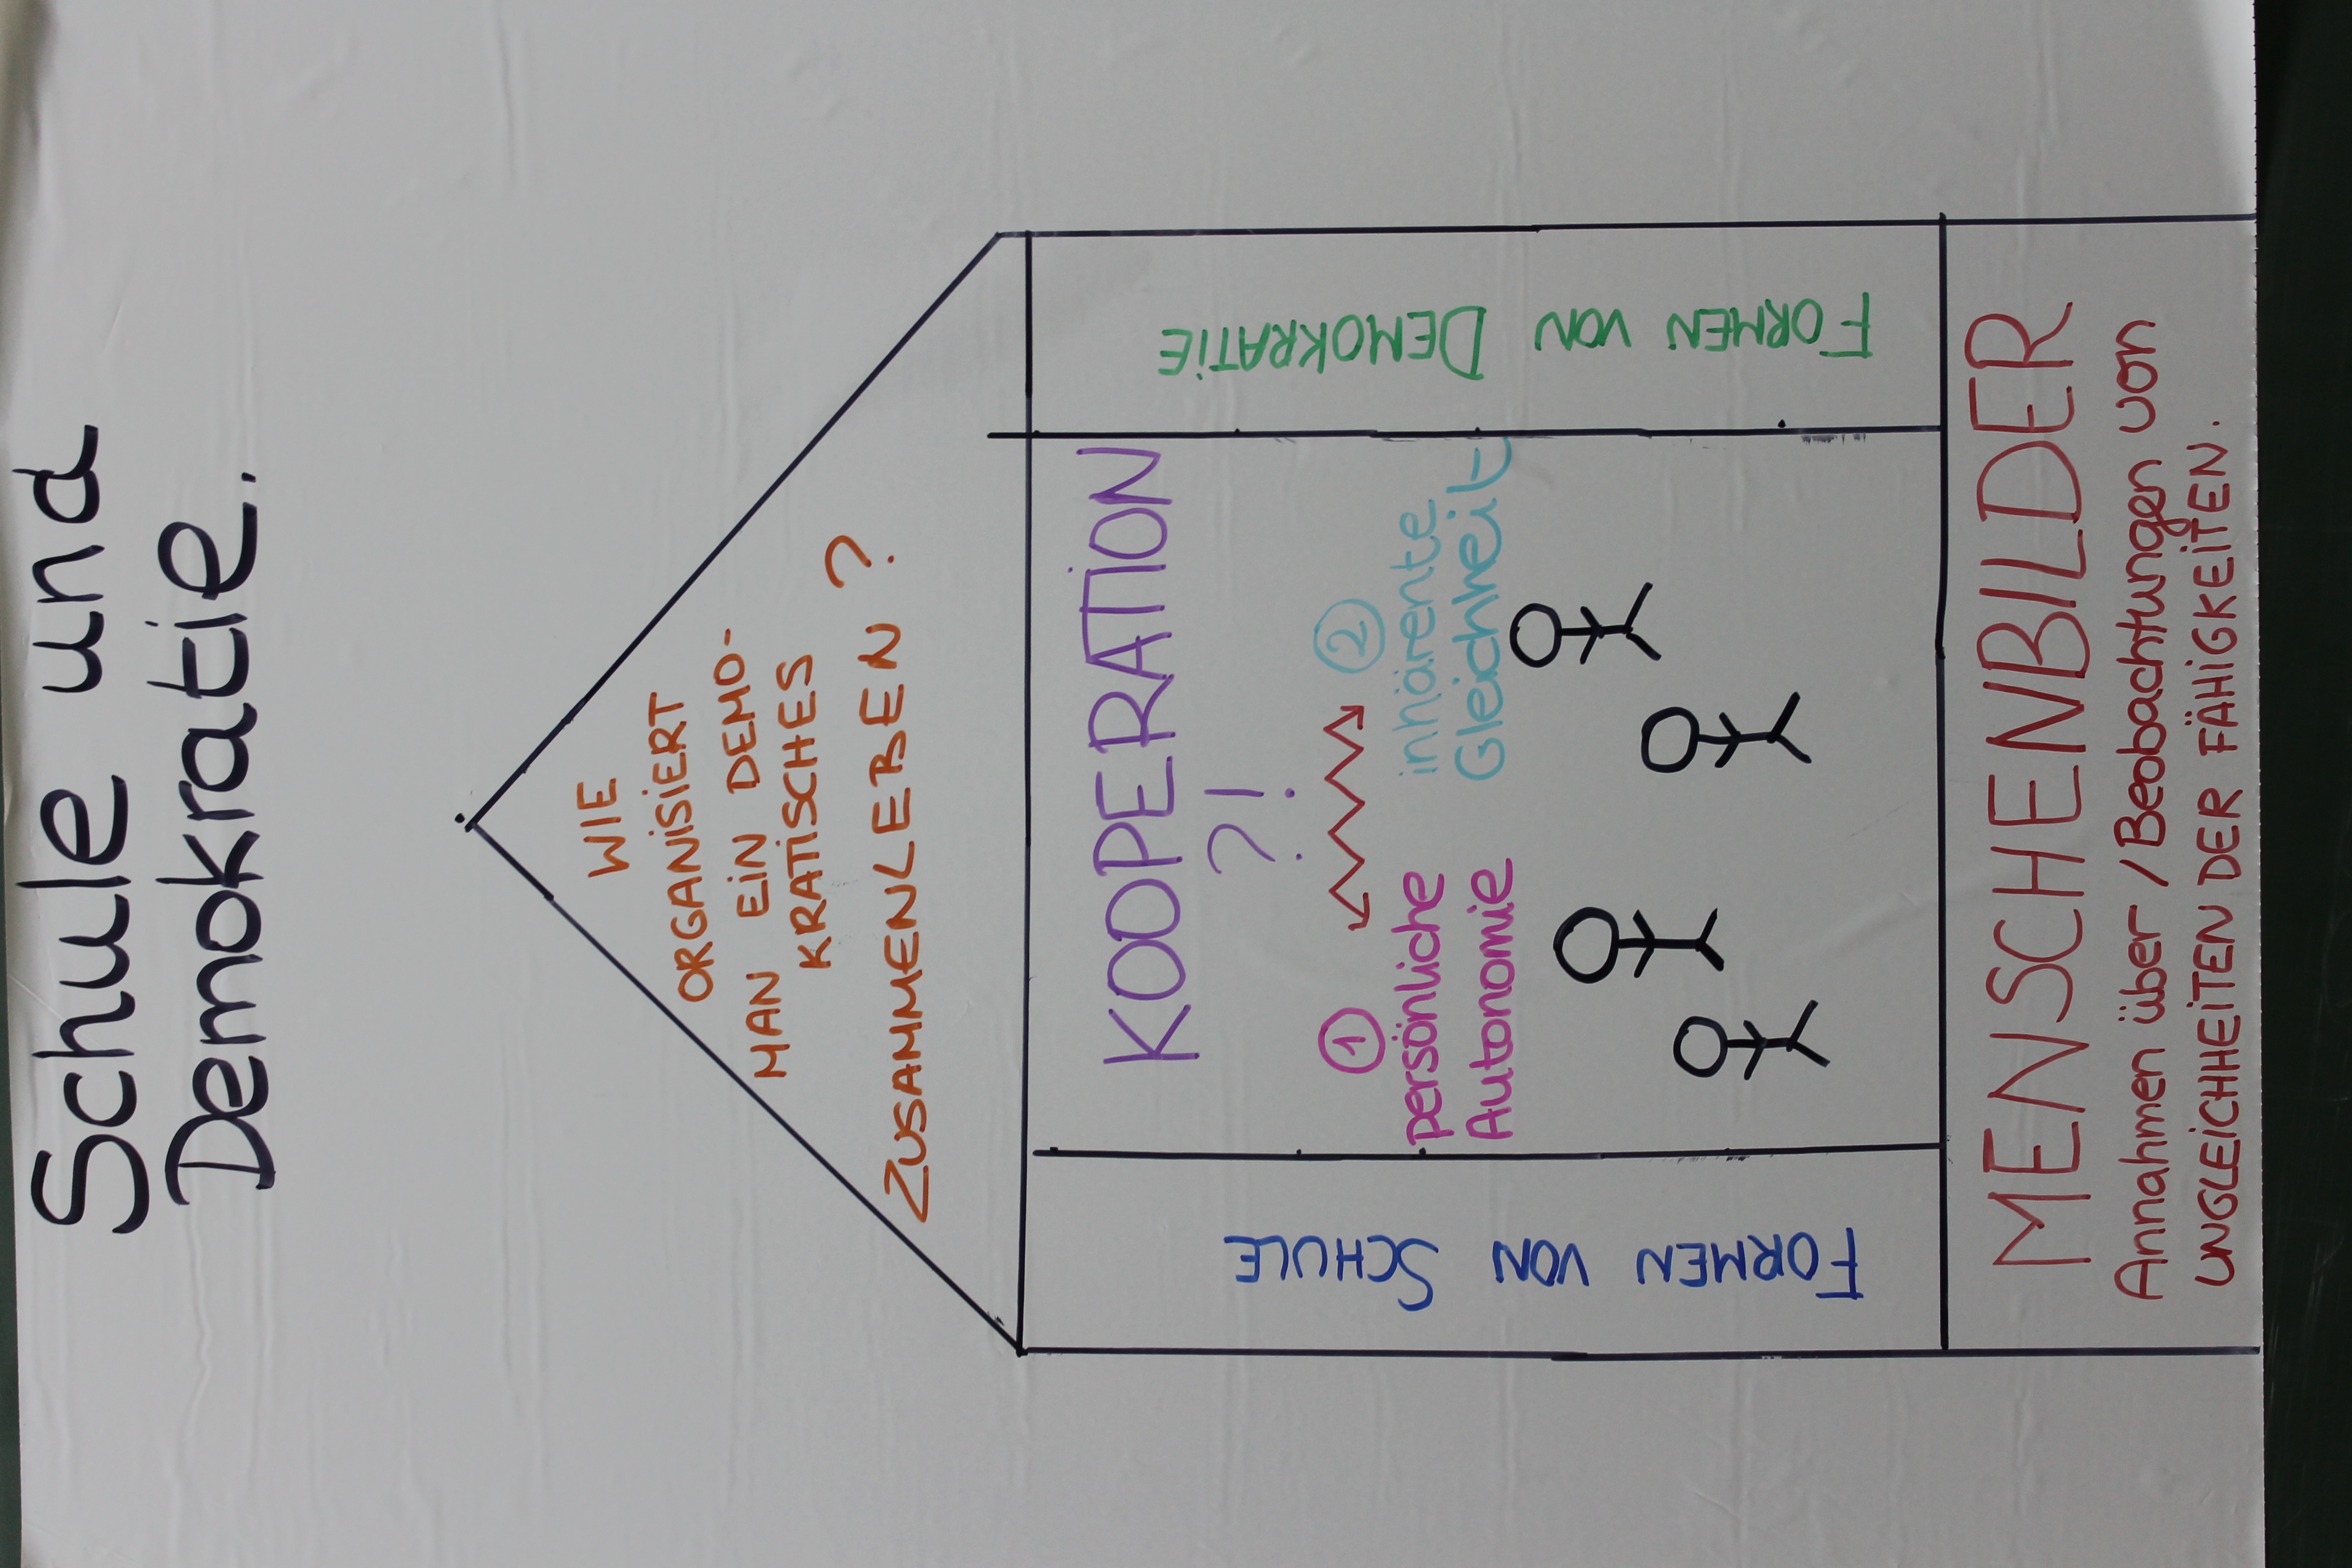
\includegraphics[width=0.9\columnwidth]{img/Kooperationshaus.JPG}
	\caption{Gemeinsame Fragen von Pädagogik und Sozialwissenschaft illustriert als Kooperationshaus}
	\label{fig:kooperationshaus}
	%\caption{Wie lässt sich menschliches Zusammenlebens bei beobachteter Ungleichheit organisieren? Ein Balanceakt zwischen inhärenter Gleichwertigkeit und persönlicher Autonomie}
	%MH FIXME: too long caption
	\end{center}
\end{dsafigure}

Nehmen wir an, dass der Mensch weder Herdentier noch Einzelgänger ist, sondern grundsätzlich in der Lage ist zu kooperieren.
Da aber (fast) jeder Mensch in eine Gesellschaft hineingeboren wird, ergibt sich zwangsläufig folgender Konflikt:
Inwiefern kann ein Mensch autonom über sich und sein Leben und Lernen entscheiden, ohne dabei die Entscheidungsfreiheit anderer und somit die inhärente Gleichheit, bzw. Gleichwertigkeit aller Menschen einzuschränken?
%VK: Ein Satz zur Kooperation ist notwendig! Ein Satz zu positiven Skalenerträgen (wird in den folgenden Beiträgen immer wieder erwähnt ohne Erklärung)

Die Aufgabe, die Balance zwischen persönlicher Autonomie und inhärenter Gleichheit zu finden, wird von unseren Autoren unterschiedlich gelöst.
Entsprechend unterschiedlich sind auch die Menschenbilder, die diesen Texten zugrunde liegen.
Sie bilden das Fundament unseres Hauses.

Den Herausforderungen des Zusammenlebens und -arbeitens nimmt sich dieser Kurs ganz konkret an:
Auf der Quellkontroll- und Versionsverwaltungsplattform \emph{github.com} versuchen wir uns an einem selbstorganisiertem Modus der Zusammenarbeit --- irgendwo zwischen Schule und Demokratie, zwischen Markt und Staat.
Dabei stellt sich uns immer wieder eine Frage:

\emph{Wie ist es also möglich, dass unterschiedliche und verschieden befähigte Menschen (auch wir auf der DSA) inhärent gleich und persönlich autonom zusammenleben?}

Unsere Einstellung zur Kursarbeit lässt sich durch ein Zitat von Martina Gedeck treffend beschreiben:

\begin{quote}
	``Im Leben geht es darum, die richtigen Fragen zu stellen und nicht darum, dauernd Antworten zu geben."\\*
	\emph{Martina Gedeck}
\end{quote}

Die richtige Frage ist gestellt, der Grundstein für unsere Brücken ist gelegt.